\documentclass[12pt,a4paper]{article}

\usepackage[utf8]{inputenc}
\usepackage[T1]{fontenc}
\usepackage[brazil]{babel}
\usepackage{lmodern}
\usepackage{microtype}
\usepackage{geometry}
\usepackage{graphicx}
\usepackage{float}
\usepackage{longtable}
\usepackage{tabularx}
\usepackage{booktabs}
\usepackage{array}
\usepackage{enumitem}
\usepackage{xcolor}
\usepackage{hyperref}
\usepackage{listings}
\usepackage{titlesec}
\usepackage{fancyhdr}
\usepackage{lastpage}
\usepackage{caption}
\usepackage{pdflscape}

\geometry{left=2.5cm,right=2.5cm,top=2.4cm,bottom=2.4cm}
\hypersetup{
    colorlinks=true,
    linkcolor=blue!55!black,
    urlcolor=blue!55!black,
    citecolor=blue!55!black,
    pdftitle={Documento de Desenvolvimento de Software - MomoRogue Engine},
    pdfauthor={Momobubu / ChatGPT}
}

\pagestyle{fancy}
\fancyhf{}
\lhead{MomoRogue Engine}
\rhead{Documento de Desenvolvimento}
\cfoot{\thepage\ de \pageref{LastPage}}

\definecolor{codebg}{RGB}{248,249,251}
\definecolor{codeframe}{RGB}{220,225,232}
\definecolor{reqblue}{RGB}{232,241,255}
\definecolor{softgreen}{RGB}{234,247,234}
\definecolor{softyellow}{RGB}{255,247,230}
\definecolor{softred}{RGB}{253,239,239}

\lstdefinestyle{momoCode}{
    backgroundcolor=\color{codebg},
    frame=single,
    rulecolor=\color{codeframe},
    basicstyle=\ttfamily\small,
    breaklines=true,
    columns=fullflexible,
    keepspaces=true,
    showstringspaces=false,
    tabsize=2,
    captionpos=b
}
\lstset{style=momoCode}

\titleformat{\section}{\Large\bfseries\color{blue!45!black}}{\thesection}{0.8em}{}
\titleformat{\subsection}{\large\bfseries\color{blue!35!black}}{\thesubsection}{0.8em}{}
\titleformat{\subsubsection}{\normalsize\bfseries}{\thesubsubsection}{0.8em}{}

\newcolumntype{Y}{>{\raggedright\arraybackslash}X}
\newcommand{\req}[1]{\textbf{#1}}

\begin{document}

\begin{titlepage}
    \centering
    \vspace*{2.0cm}
    {\Huge\bfseries Documento de Desenvolvimento de Software\\[0.3cm]}
    {\LARGE\bfseries MomoRogue Engine\\[0.4cm]}
    {\large Engine especializada para jogos roguelike em C\#, SadConsole, scripting e exportação para executável/instalador\\[1.5cm]}
    \vfill
    \begin{tabular}{rl}
        \textbf{Versão:} & 0.1 - Documento inicial de arquitetura e requisitos \\
        \textbf{Data:} & 11 de junho de 2026 \\
        \textbf{Plataforma alvo inicial:} & Windows x64 \\
        \textbf{Tecnologias base:} & C\#, .NET, SadConsole, Avalonia, Roslyn, WiX \\
        \textbf{Status:} & Planejamento técnico para MVP \\
    \end{tabular}
    \vfill
    {\large Salvador - BA\\}
\end{titlepage}

\tableofcontents
\newpage

\section{Introdução}

Este documento especifica o desenvolvimento da \textbf{MomoRogue Engine}, uma engine própria, especializada em jogos \textit{roguelike} 2D baseados em grade. O objetivo não é criar uma engine genérica no estilo Unity, Godot ou Unreal, mas uma plataforma focada em um domínio menor e mais controlável: mapas tile-based, entidades, turnos, geração procedural, campo de visão, pathfinding, scripts de gameplay e exportação do jogo final para executável ou instalador.

A decisão técnica central é usar \textbf{C\#} como linguagem principal e \textbf{SadConsole} como camada de renderização/input. A lógica da engine deve permanecer desacoplada do SadConsole, permitindo que a engine seja testada sem interface gráfica e, futuramente, possa receber outro renderizador. O SadConsole entra como adaptador visual para desenhar tiles, glyphs, spritesheets e interfaces textuais/semigráficas.

\subsection{Objetivo geral}

Desenvolver uma engine modular para criação de jogos roguelike, com suporte a edição de projeto, programação em C\#, visual scripting, execução em runtime e exportação automatizada para formatos distribuíveis.

\subsection{Objetivos específicos}

\begin{enumerate}[label=\alph*)]
    \item Definir uma arquitetura modular e testável para o núcleo da engine.
    \item Implementar um runtime capaz de carregar projetos de jogo, assets, dados e scripts.
    \item Integrar SadConsole como renderizador tile-based e camada de input.
    \item Permitir scripts em C\# compilados junto ao projeto do jogo.
    \item Permitir visual scripting por grafo, inicialmente convertido para C\# gerado.
    \item Criar um editor desktop para gerenciar projetos, dados, assets e exportação.
    \item Criar um build tool capaz de gerar executável, pasta portable e instalador.
    \item Manter a engine especializada em roguelikes para reduzir escopo e aumentar viabilidade.
\end{enumerate}

\section{Escopo do Produto}

\subsection{Produto proposto}

A MomoRogue Engine será composta por quatro partes principais:

\begin{itemize}
    \item \textbf{Engine}: biblioteca com regras, entidades, turnos, mapas, geração procedural, FOV, pathfinding, save/load e sistemas de jogo.
    \item \textbf{Runtime}: aplicação base que executa jogos criados com a engine.
    \item \textbf{Editor}: ferramenta desktop para criação e configuração de projetos.
    \item \textbf{Build Tool}: ferramenta de empacotamento e exportação para executável, ZIP portable e instalador.
\end{itemize}

\subsection{Fora do escopo inicial}

Para manter o projeto viável, ficam fora do MVP:

\begin{itemize}
    \item Física 2D/3D genérica.
    \item Animação pixel-perfect complexa fora do grid.
    \item Editor visual completo equivalente a Unity/Godot.
    \item Multiplayer online.
    \item Marketplace de assets ou mods.
    \item Suporte mobile no primeiro ciclo.
    \item Scripting não confiável com sandbox robusta.
\end{itemize}

\section{Justificativa Técnica da Stack}

A stack proposta privilegia produtividade, integração com tooling moderno e aderência ao tipo de jogo. SadConsole é adequado porque roguelikes geralmente operam em grade, usando caracteres, glyphs ou tiles. C\# e .NET facilitam organização modular, reflexão, geração de código, serialização, integração com Roslyn e publicação multiplataforma.

\begin{longtable}{p{3.3cm}p{4.6cm}p{6.4cm}}
\toprule
\textbf{Camada} & \textbf{Escolha} & \textbf{Motivo} \\
\midrule
Linguagem & C\# & Boa ergonomia, tipagem forte, tooling maduro, integração com .NET SDK e Roslyn. \\
Runtime/base & .NET & Permite publicar aplicações self-contained e single-file com \texttt{dotnet publish}. \\
Renderização & SadConsole & Adequado a jogos ASCII, ANSI, tile-based e roguelike. \\
Host gráfico & MonoGame via SadConsole & Permite janela, input e renderização 2D por backend já suportado. \\
Editor & Avalonia UI & Framework desktop .NET multiplataforma com XAML, MVVM e boa separação de interface/lógica. \\
Scripting & Roslyn / Microsoft.CodeAnalysis & Permite compilação/análise de scripts C\# e geração de assemblies. \\
Instalador & WiX Toolset & Geração de MSI/instaladores Windows com controle fino do pacote. \\
Dados & JSON & Simples, legível, versionável e suficiente para entidades, itens, configs e grafos. \\
\bottomrule
\end{longtable}

\section{Visão Geral da Arquitetura}

A arquitetura deve evitar dependência direta entre gameplay e renderizador. O núcleo da engine não deve conhecer SadConsole. Ele apenas expõe estado, eventos e comandos. O adaptador SadConsole lê esse estado e desenha o mundo.

\begin{figure}[H]
    \centering
    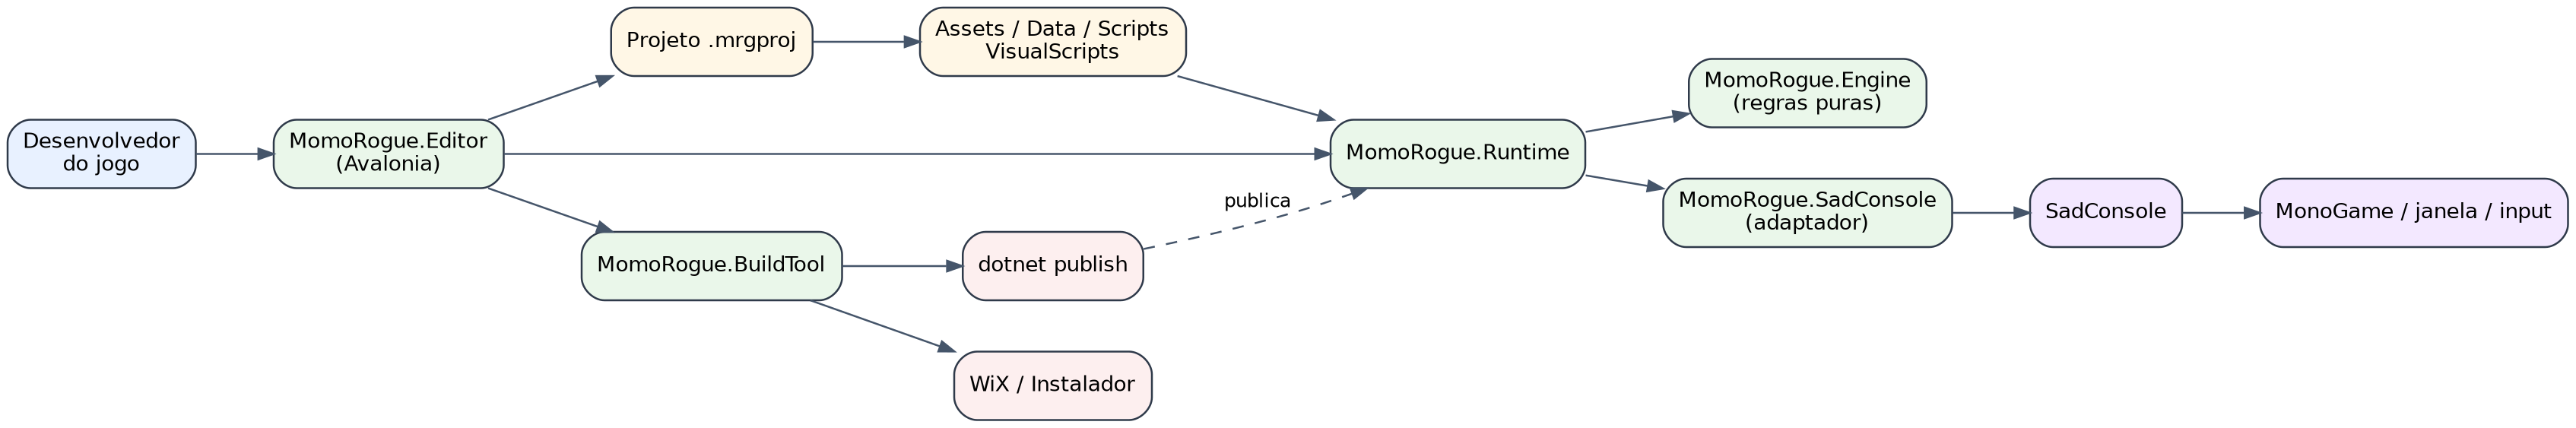
\includegraphics[width=0.98\textwidth]{../rendered/01_contexto_arquitetura.png}
    \caption{Contexto geral da arquitetura proposta.}
\end{figure}

\subsection{Princípio arquitetural principal}

\begin{quote}
\textit{SadConsole é tela; MomoRogue.Engine é regra de jogo.}
\end{quote}

Essa separação reduz acoplamento e facilita testes automatizados. A engine deve conseguir processar turnos, combate, movimentação, geração procedural e saves sem abrir uma janela gráfica.

\subsection{Organização da solução}

\begin{lstlisting}[language={},caption={Estrutura inicial da solução C\#.}]
MomoRogue/
  src/
    MomoRogue.Engine/
    MomoRogue.SadConsole/
    MomoRogue.Runtime/
    MomoRogue.Editor/
    MomoRogue.BuildTool/
  templates/
    BasicRoguelikeProject/
  samples/
    DungeonSample/
    SciFiSample/
  tests/
    MomoRogue.Engine.Tests/
    MomoRogue.BuildTool.Tests/
  docs/
    diagrams/
\end{lstlisting}

\section{Módulos da Engine}

\begin{figure}[H]
    \centering
    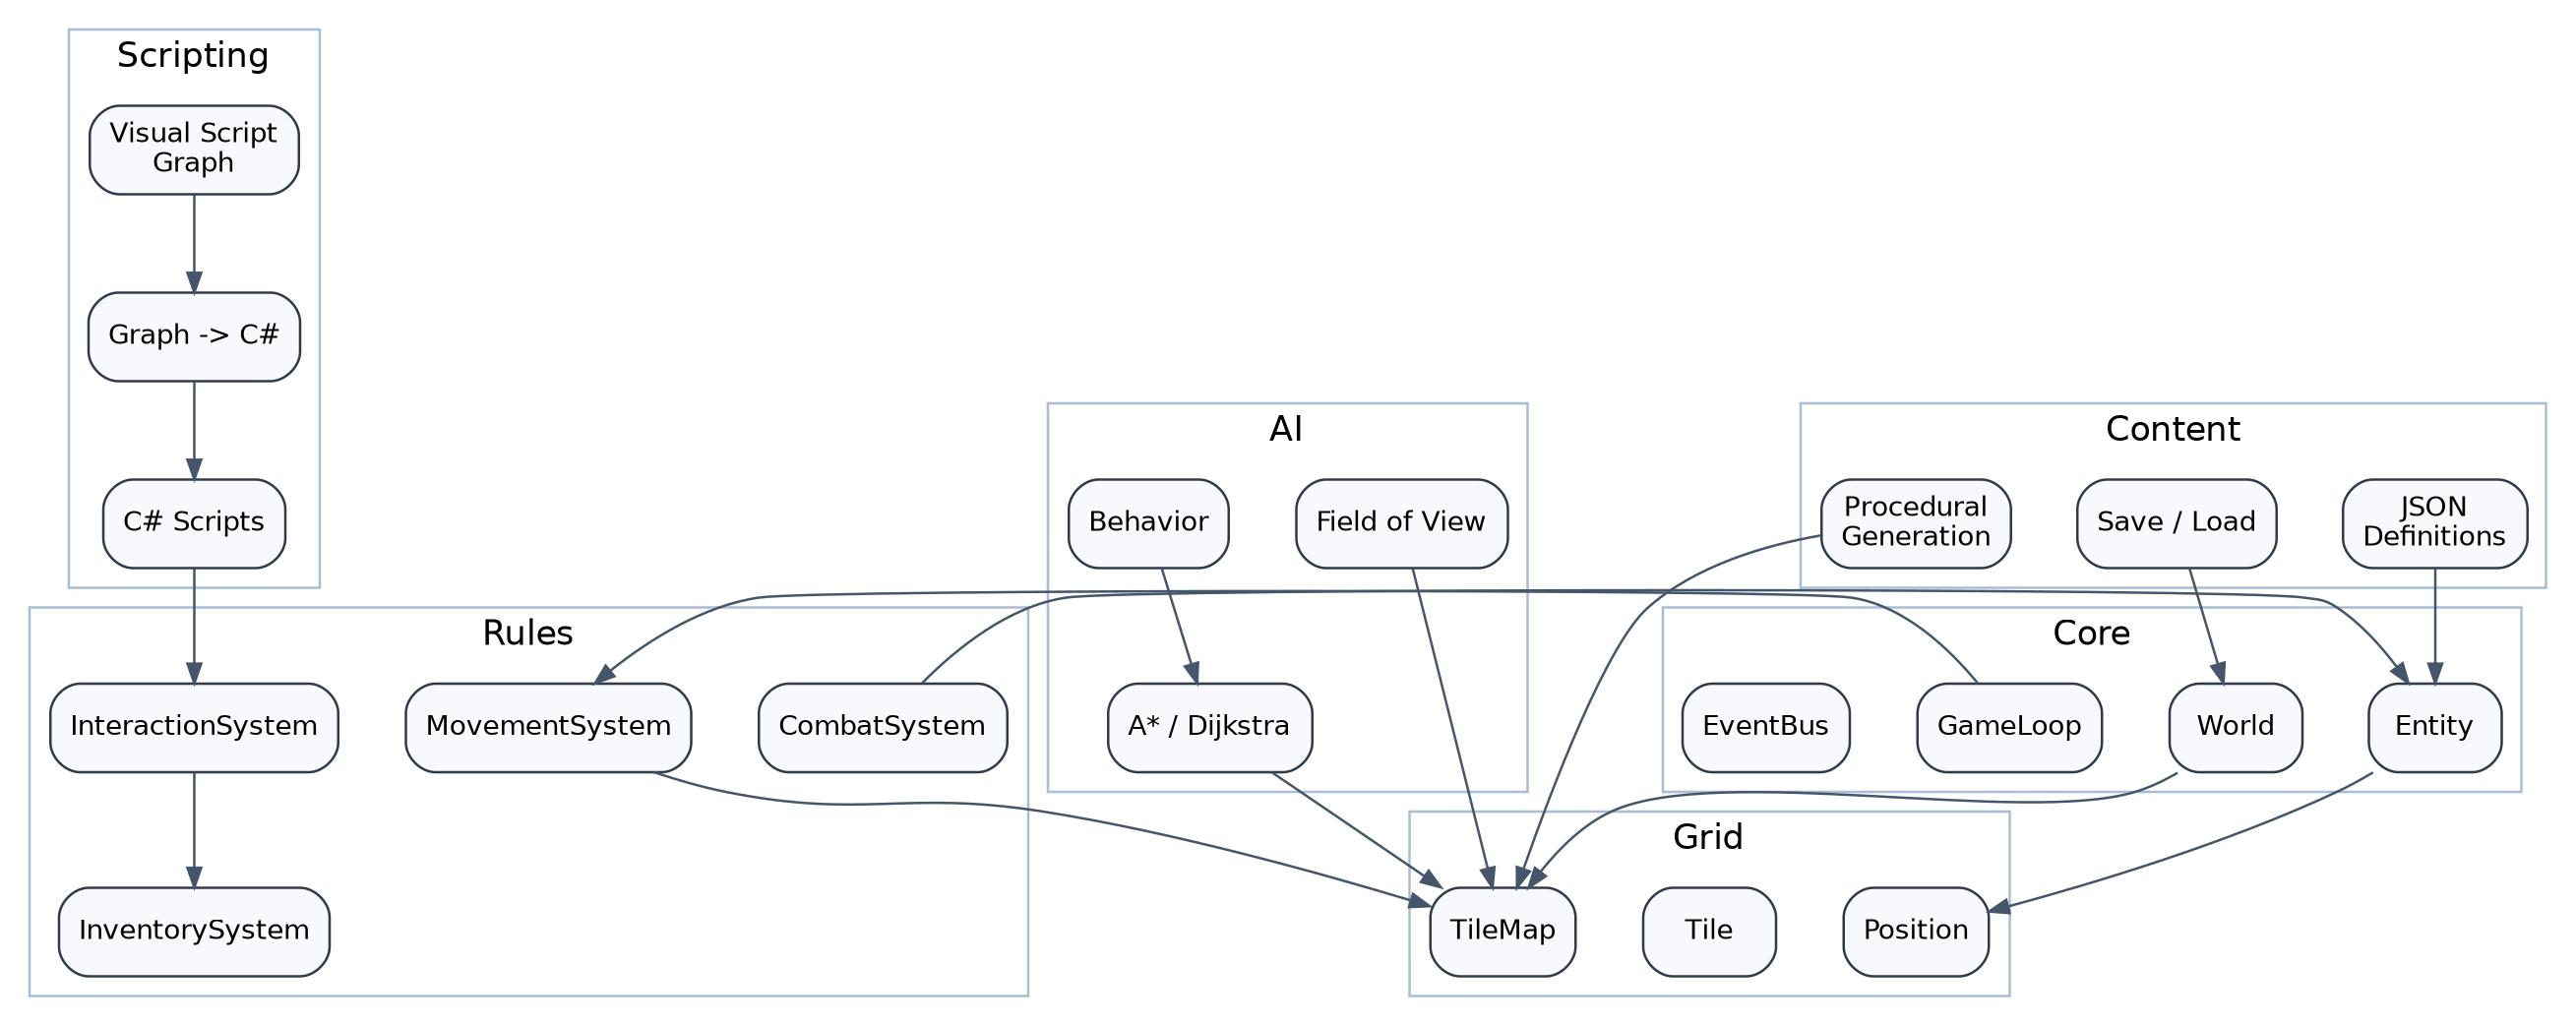
\includegraphics[width=0.98\textwidth]{../rendered/02_modulos_engine.png}
    \caption{Módulos internos da engine.}
\end{figure}

\subsection{MomoRogue.Engine}

Biblioteca pura com as regras e estruturas principais. Não deve depender de SadConsole, Avalonia ou UI.

\begin{itemize}
    \item \textbf{Core}: loop abstrato, mundo, entidades, componentes e eventos.
    \item \textbf{Grid}: tilemap, posição, direção, tamanho, colisão e visibilidade.
    \item \textbf{TurnBased}: gerência de turnos, energia, velocidade e ações.
    \item \textbf{Rules}: movimento, combate, inventário, interação e uso de itens.
    \item \textbf{AI}: comportamentos, pathfinding, Dijkstra map e FOV.
    \item \textbf{ProcGen}: geração procedural de salas, corredores, cavernas e andares.
    \item \textbf{Scripting}: contrato para scripts C\# e visual scripts.
    \item \textbf{Persistence}: save/load e serialização do estado de jogo.
\end{itemize}

\subsection{MomoRogue.SadConsole}

Adaptador responsável por traduzir estado da engine para tela.

\begin{itemize}
    \item Renderização de tilemap.
    \item Renderização de entidades por glyph/tile.
    \item Camadas de UI: log, inventário, status, menu.
    \item Tradução de input para comandos da engine.
    \item Carregamento de spritesheets/tilesets compatíveis com SadConsole.
\end{itemize}

\subsection{MomoRogue.Runtime}

Aplicação que executa o jogo final. Ela carrega o pacote do jogo, inicializa a engine, conecta o renderer e inicia o loop.

\subsection{MomoRogue.Editor}

Aplicação desktop para criar e configurar projetos. O editor não deve ser obrigatório para executar o jogo. Ele é uma ferramenta de produção.

\subsection{MomoRogue.BuildTool}

Ferramenta de linha de comando ou serviço interno do editor responsável por validar projeto, gerar código, compilar scripts, copiar assets e executar publicação.

\section{Modelo de Projeto do Jogo}

Um jogo criado na engine deve ser uma pasta versionável, contendo dados, scripts, assets e configuração.

\begin{lstlisting}[language={},caption={Estrutura de um projeto de jogo.}]
MeuJogo/
  game.mrgproj
  Assets/
    Tilesets/
      dungeon_16x16.png
    Audio/
    Fonts/
  Data/
    actors.json
    items.json
    maps.json
    factions.json
  Scripts/
    PlayerController.cs
    GoblinAI.cs
    FireballSpell.cs
  VisualScripts/
    door_interaction.graph.json
    boss_intro.graph.json
  Build/
\end{lstlisting}

\subsection{Arquivo game.mrgproj}

\begin{lstlisting}[language={},caption={Exemplo de configuração do projeto.}]
{
  "name": "Meu Roguelike",
  "id": "meu-roguelike",
  "version": "0.1.0",
  "engineVersion": "0.1.0",
  "entryScene": "dungeon_start",
  "tileSize": 16,
  "target": "win-x64",
  "outputType": "portable",
  "scripting": {
    "compileCSharpScripts": true,
    "compileVisualScripts": true
  }
}
\end{lstlisting}

\section{Requisitos Funcionais}

\begin{longtable}{p{2.1cm}p{4.1cm}p{7.8cm}}
\toprule
\textbf{ID} & \textbf{Nome} & \textbf{Descrição} \\
\midrule
\req{RF-01} & Criar projeto & O editor deve permitir criar um novo projeto roguelike a partir de um template. \\
\req{RF-02} & Abrir projeto & O editor e o runtime devem carregar um projeto existente por meio do arquivo \texttt{game.mrgproj}. \\
\req{RF-03} & Renderizar mapa & O runtime deve renderizar um mapa baseado em grade usando SadConsole. \\
\req{RF-04} & Suportar tiles/glyphs & A engine deve permitir representar entidades e tiles por glyphs, caracteres ou sprites de tileset. \\
\req{RF-05} & Gerenciar entidades & A engine deve criar, consultar, atualizar e remover entidades do mundo. \\
\req{RF-06} & Componentes & Entidades devem poder receber componentes como posição, renderização, vida, inventário, AI e colisão. \\
\req{RF-07} & Movimento e colisão & A engine deve validar movimento com base em limites do mapa, paredes, entidades bloqueantes e regras de interação. \\
\req{RF-08} & Sistema de turnos & O runtime deve executar turnos do jogador e de entidades controladas por IA. \\
\req{RF-09} & Combate básico & A engine deve fornecer regras mínimas de ataque, dano, vida e morte. \\
\req{RF-10} & Geração procedural & A engine deve gerar dungeons simples com salas e corredores. \\
\req{RF-11} & Campo de visão & A engine deve calcular tiles visíveis, explorados e desconhecidos. \\
\req{RF-12} & Pathfinding & A engine deve oferecer caminho para IA por A* ou Dijkstra map. \\
\req{RF-13} & Scripts C\# & O projeto deve aceitar scripts C\# compilados junto ao jogo. \\
\req{RF-14} & Visual scripting & O editor deve permitir criar grafos visuais que geram código C\#. \\
\req{RF-15} & Playtest & O editor deve permitir executar o jogo em modo de teste. \\
\req{RF-16} & Exportar executável & O build tool deve gerar executável Windows x64 a partir do projeto. \\
\req{RF-17} & Exportar ZIP portable & O build tool deve gerar uma pasta ou arquivo ZIP executável sem instalação. \\
\req{RF-18} & Gerar instalador & O build tool deve gerar instalador MSI/EXE em ciclo posterior ao MVP inicial. \\
\req{RF-19} & Save/load & O runtime deve salvar e carregar estado do jogo. \\
\req{RF-20} & Logs de erro & Editor e build tool devem exibir erros de validação, script e exportação. \\
\bottomrule
\end{longtable}

\section{Requisitos Não Funcionais}

\begin{longtable}{p{2.1cm}p{4.1cm}p{7.8cm}}
\toprule
\textbf{ID} & \textbf{Categoria} & \textbf{Descrição} \\
\midrule
\req{RNF-01} & Modularidade & O núcleo da engine deve ser independente de SadConsole, Avalonia e BuildTool. \\
\req{RNF-02} & Testabilidade & Regras de jogo devem ser testáveis por testes unitários sem renderização gráfica. \\
\req{RNF-03} & Desempenho & O MVP deve manter 60 FPS na renderização de mapas pequenos/médios, mesmo com turnos processados sob demanda. \\
\req{RNF-04} & Portabilidade & A arquitetura deve permitir exportação futura para Linux e macOS, mesmo que o MVP foque Windows x64. \\
\req{RNF-05} & Manutenibilidade & Cada módulo deve ter responsabilidade clara e baixo acoplamento. \\
\req{RNF-06} & Reprodutibilidade & Geração procedural deve aceitar seed para reproduzir mapas. \\
\req{RNF-07} & Segurança & Scripts C\# devem ser tratados como código confiável no MVP; mods não confiáveis exigem política futura de sandbox. \\
\req{RNF-08} & Observabilidade & Build e runtime devem gerar logs legíveis de erro, warning e eventos importantes. \\
\req{RNF-09} & Versionamento & Projetos devem declarar versão da engine e permitir migração futura de schema. \\
\req{RNF-10} & Usabilidade & O editor deve priorizar fluxos simples: criar projeto, editar dados, testar e exportar. \\
\bottomrule
\end{longtable}

\section{Casos de Uso}

\begin{figure}[H]
    \centering
    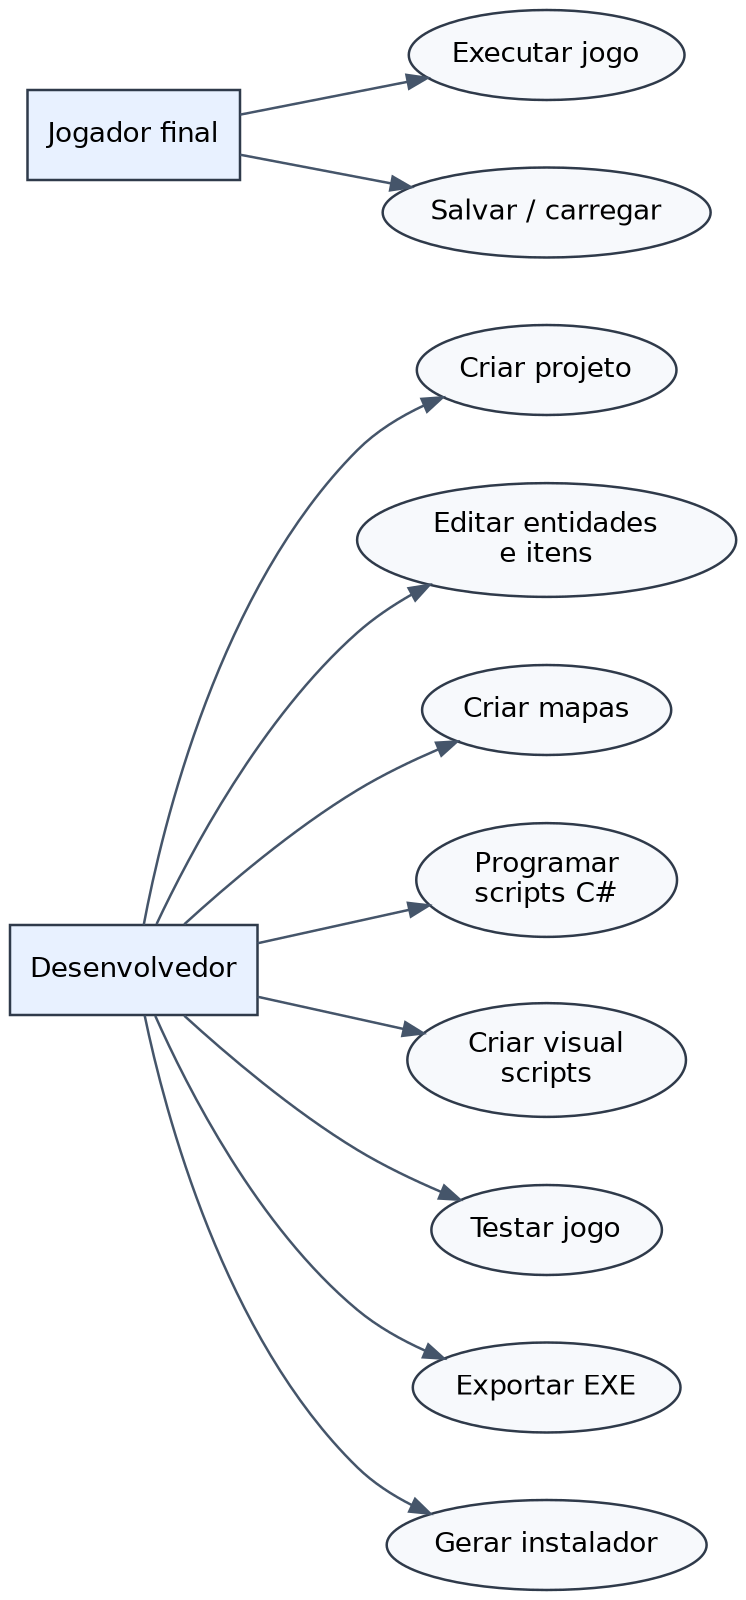
\includegraphics[height=0.68\textheight,keepaspectratio]{../rendered/08_casos_de_uso.png}
    \caption{Casos de uso principais.}
\end{figure}

\subsection{UC-01 - Criar projeto}

\textbf{Ator principal}: Desenvolvedor.\\
\textbf{Fluxo}: abre o editor, escolhe template, define nome, pasta e configurações iniciais.\\
\textbf{Resultado}: pasta de projeto criada com estrutura inicial, arquivos JSON, scripts exemplo e assets mínimos.

\subsection{UC-02 - Programar comportamento em C\#}

\textbf{Ator principal}: Desenvolvedor.\\
\textbf{Fluxo}: cria um arquivo \texttt{.cs} na pasta \texttt{Scripts/}, implementa uma classe derivada de contrato da engine, compila pelo editor/build tool.\\
\textbf{Resultado}: o comportamento fica disponível para entidades do jogo.

\subsection{UC-03 - Criar visual script}

\textbf{Ator principal}: Desenvolvedor.\\
\textbf{Fluxo}: abre editor de grafos, conecta eventos, condições e ações.\\
\textbf{Resultado}: o grafo é salvo como JSON e convertido para C\# gerado no build.

\subsection{UC-04 - Exportar jogo}

\textbf{Ator principal}: Desenvolvedor.\\
\textbf{Fluxo}: seleciona perfil de build, valida projeto, gera código, compila scripts, publica runtime e empacota.\\
\textbf{Resultado}: executável, pasta portable ou instalador.

\section{Pipeline de Build e Exportação}

\begin{figure}[H]
    \centering
    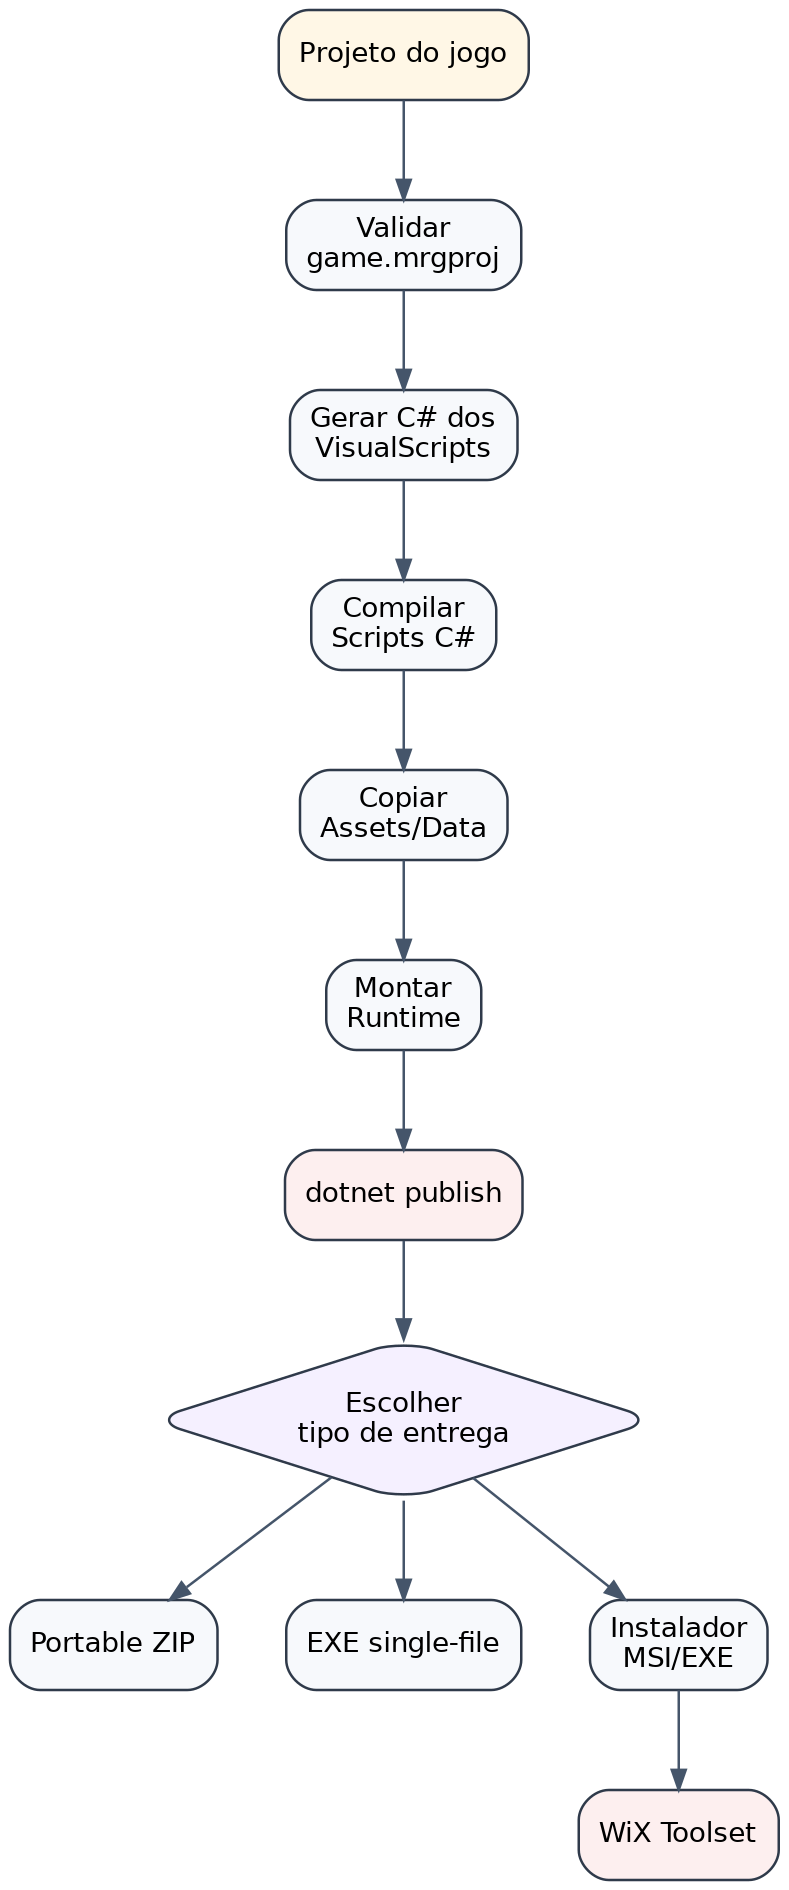
\includegraphics[height=0.68\textheight,keepaspectratio]{../rendered/03_pipeline_build.png}
    \caption{Pipeline de exportação do projeto para executável ou instalador.}
\end{figure}

\subsection{Estratégia de build}

A engine não precisa implementar um compilador próprio. Ela deve orquestrar o tooling do .NET:

\begin{enumerate}
    \item Validar o arquivo \texttt{game.mrgproj}.
    \item Validar JSONs de dados.
    \item Gerar C\# a partir de visual scripts.
    \item Criar ou atualizar o projeto \texttt{.csproj} temporário do jogo.
    \item Compilar scripts C\# e código gerado.
    \item Copiar assets e dados para a saída.
    \item Executar \texttt{dotnet publish} com perfil definido.
    \item Opcionalmente executar empacotamento MSI/EXE por WiX.
\end{enumerate}

\subsection{Comando base de publicação}

\begin{lstlisting}[language={},caption={Comando conceitual de exportação Windows x64.}]
dotnet publish MeuJogo.Runtime.csproj \
  -c Release \
  -r win-x64 \
  --self-contained true \
  /p:PublishSingleFile=true \
  /p:PublishTrimmed=false
\end{lstlisting}

\subsection{Tipos de entrega}

\begin{longtable}{p{3.4cm}p{4.4cm}p{6.2cm}}
\toprule
\textbf{Tipo} & \textbf{Quando usar} & \textbf{Observações} \\
\midrule
Pasta portable & MVP e testes & Mais simples; facilita debugar assets e DLLs. \\
ZIP portable & Distribuição simples & Compacta a pasta publicada. \\
EXE single-file & Distribuição limpa & Pode exigir cuidado com assets externos e extração. \\
Instalador MSI/EXE & Distribuição final & Deve ser feito após estabilidade do runtime e do formato do projeto. \\
\bottomrule
\end{longtable}

\section{Runtime e Fluxo de Turno}

O runtime executa um ciclo orientado a ações. O jogo não precisa atualizar lógica pesada a cada frame; a lógica de roguelike geralmente avança quando o jogador executa uma ação.

\begin{figure}[H]
    \centering
    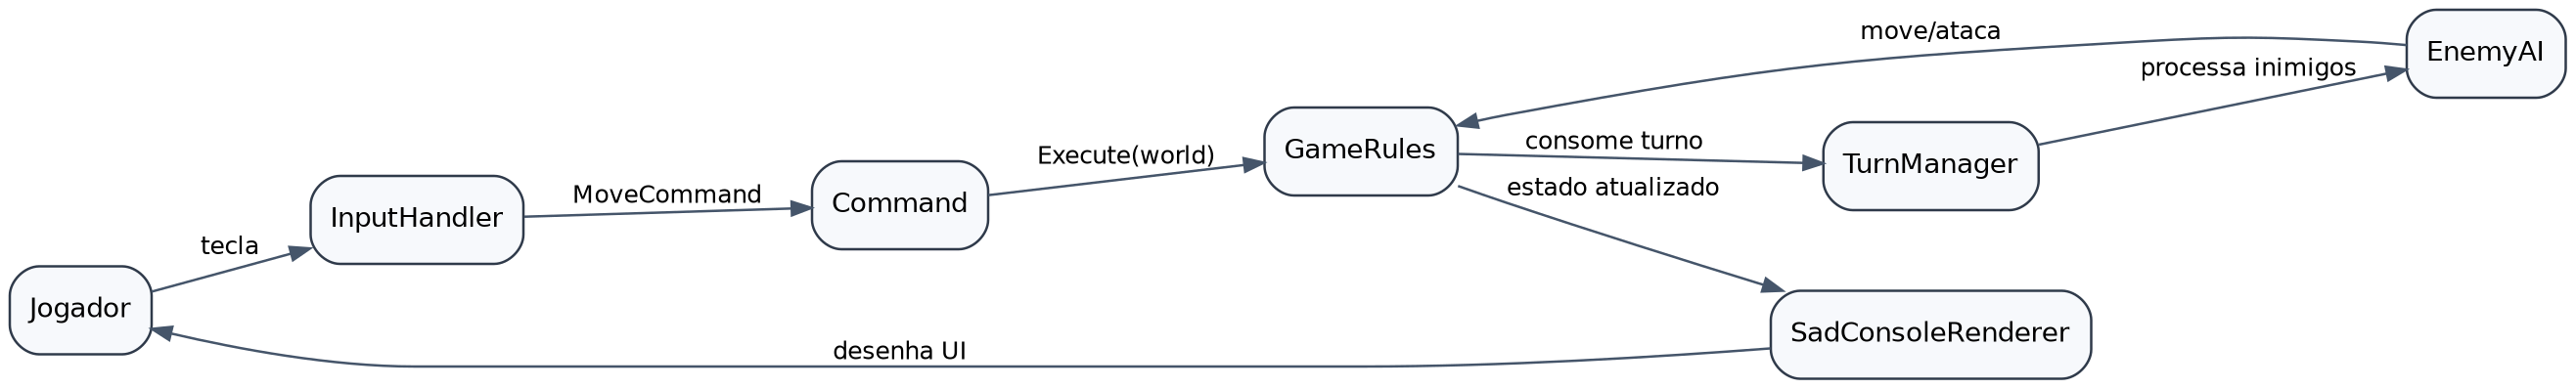
\includegraphics[width=0.95\textwidth]{../rendered/04_sequence_turno.png}
    \caption{Sequência de processamento de um turno.}
\end{figure}

\subsection{Estados do runtime}

\begin{figure}[H]
    \centering
    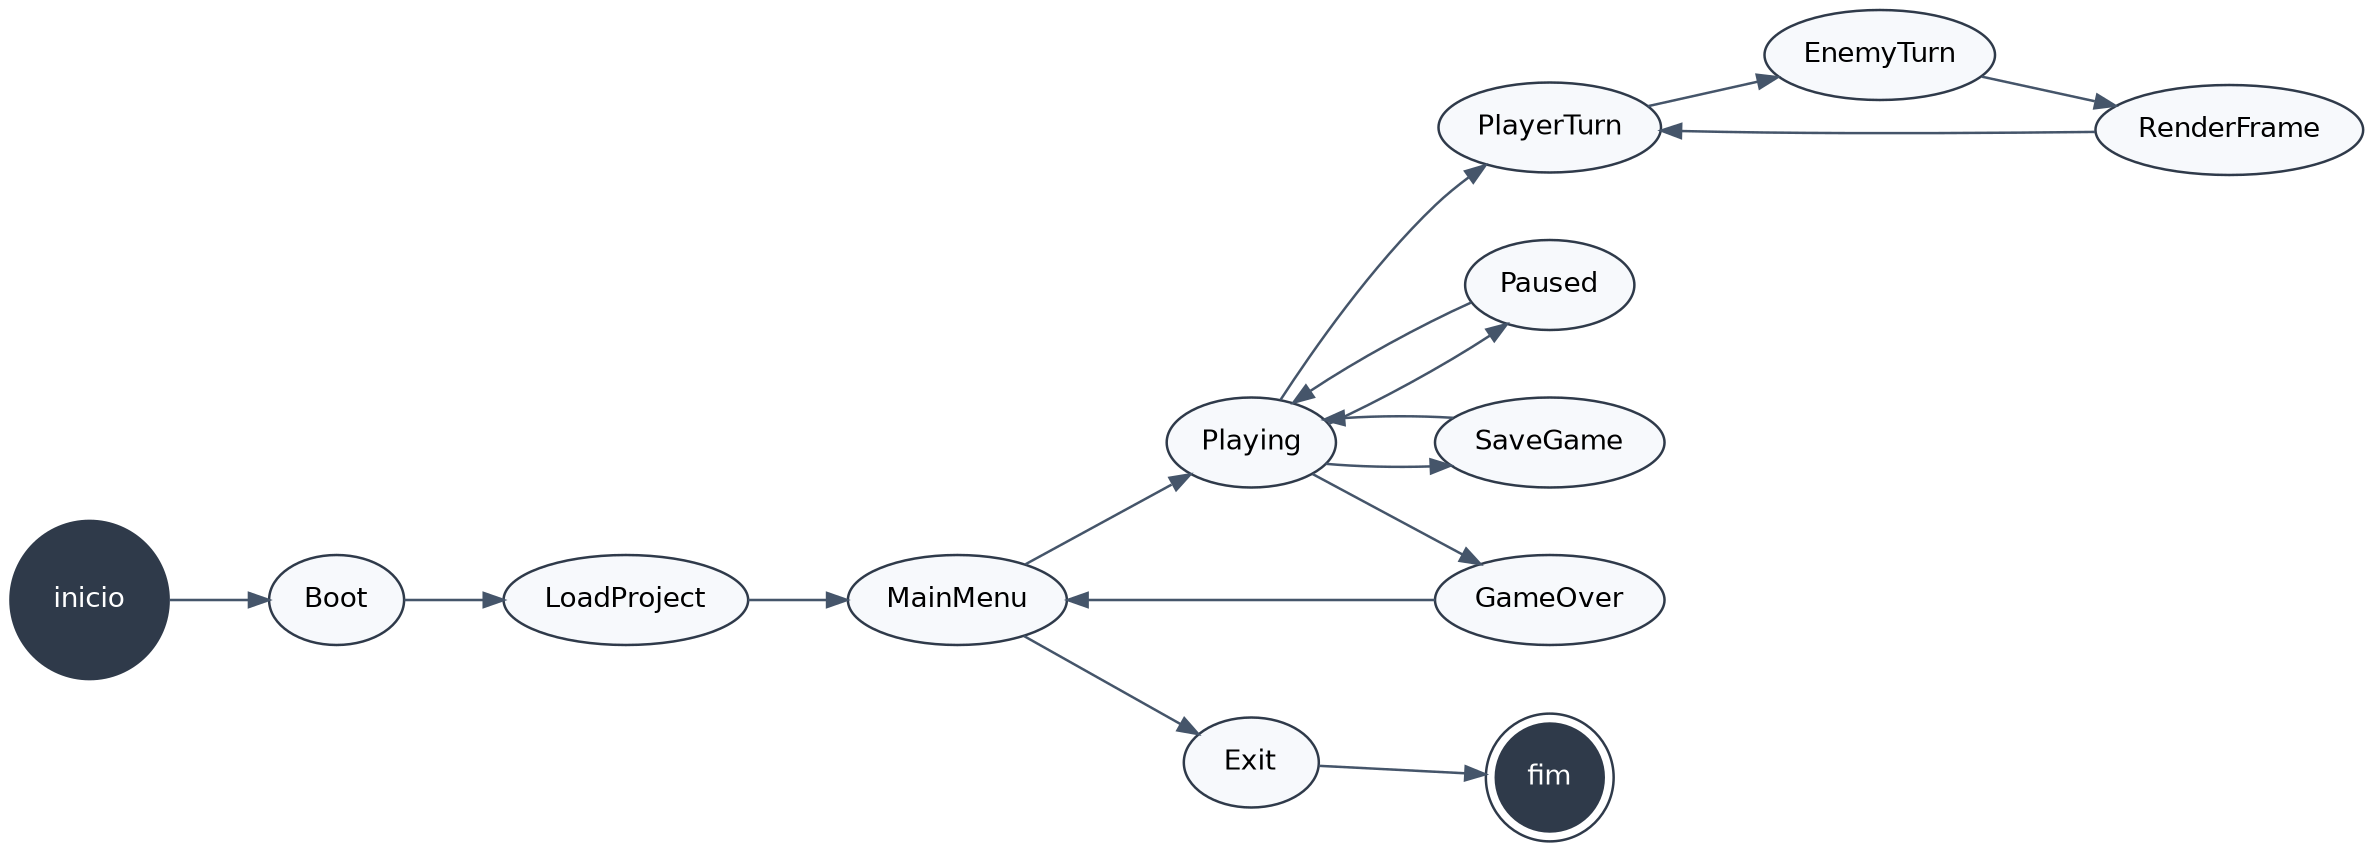
\includegraphics[width=0.95\textwidth]{../rendered/07_estado_runtime.png}
    \caption{Estados principais do runtime.}
\end{figure}

\section{Modelo de Classes Inicial}

A engine deve começar simples, com um modelo de entidades e componentes pragmático. Não é necessário implementar ECS puro no MVP. O ideal é usar entidades com componentes tipados e sistemas bem separados.

\begin{figure}[H]
    \centering
    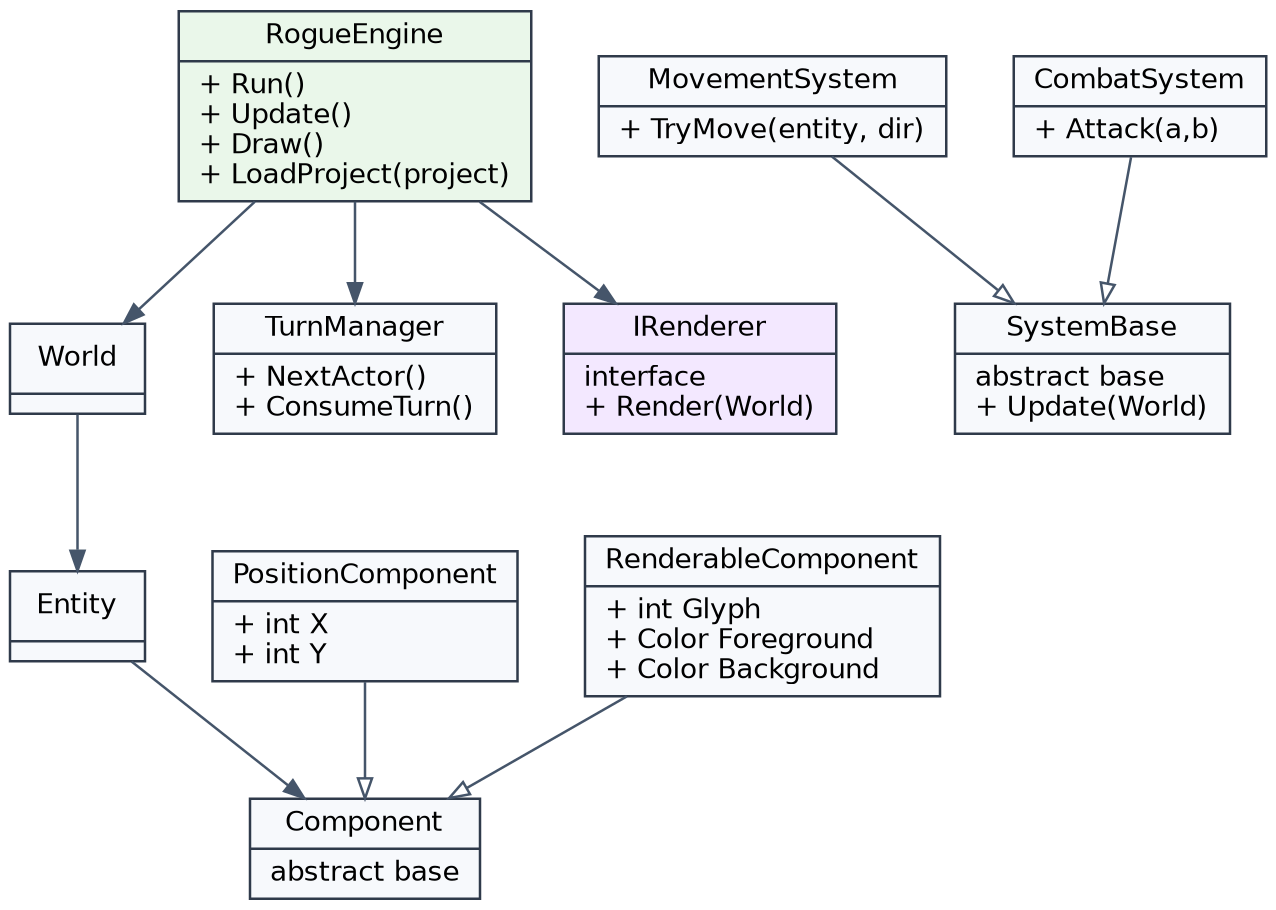
\includegraphics[width=0.98\textwidth]{../rendered/05_class_core.png}
    \caption{Modelo conceitual de classes do núcleo da engine.}
\end{figure}

\subsection{Exemplo de contratos em C\#}

\begin{lstlisting}[language={[Sharp]C},caption={Exemplo conceitual de contrato de renderer.}]
public interface IRenderer
{
    void Render(World world);
}

public sealed class RogueEngine
{
    private readonly World world;
    private readonly IRenderer renderer;
    private readonly TurnManager turnManager;

    public void Update(ICommand? command)
    {
        if (command is null)
            return;

        command.Execute(world);
        turnManager.ProcessNonPlayerActors(world);
    }

    public void Draw()
    {
        renderer.Render(world);
    }
}
\end{lstlisting}

\section{Scripting em C\#}

\subsection{Estratégia inicial}

O MVP deve priorizar scripts C\# compilados junto com o jogo, não execução dinâmica irrestrita em runtime. Isso é mais simples, performático e previsível.

\begin{lstlisting}[language={[Sharp]C},caption={Exemplo de comportamento de inimigo em C\#.}]
using MomoRogue.Engine;

public sealed class GoblinAI : ActorBehavior
{
    public override void OnTurn(Actor self, World world)
    {
        Entity player = world.Player;

        if (self.Position.DistanceTo(player.Position) <= 1)
        {
            self.Attack(player);
            return;
        }

        self.MoveToward(player.Position);
    }
}
\end{lstlisting}

\subsection{Regras para scripts}

\begin{itemize}
    \item Scripts devem implementar interfaces ou herdar classes abstratas da engine.
    \item Scripts não devem acessar diretamente SadConsole.
    \item O build tool deve compilar scripts e exibir erros com arquivo, linha e coluna.
    \item Scripts do MVP são considerados código confiável do próprio desenvolvedor.
    \item Suporte a mods externos deve ser tratado em fase posterior.
\end{itemize}

\section{Visual Scripting}

O visual scripting deve ser implementado como um grafo que gera C\#. Essa decisão evita criar um interpretador visual complexo no primeiro ciclo e mantém a execução final dentro do ecossistema C\#.

\begin{figure}[H]
    \centering
    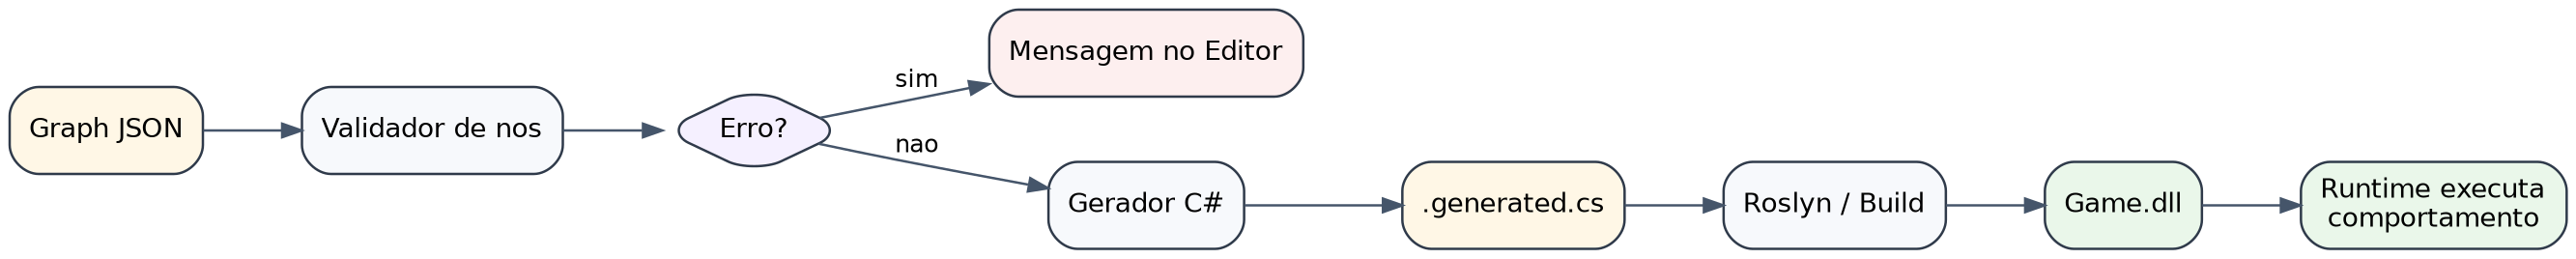
\includegraphics[width=0.95\textwidth]{../rendered/06_visual_script.png}
    \caption{Fluxo de compilação de visual script.}
\end{figure}

\subsection{Modelo do grafo}

\begin{lstlisting}[language={},caption={Exemplo de grafo visual salvo em JSON.}]
{
  "name": "DoorInteraction",
  "event": "OnInteract",
  "nodes": [
    { "id": "1", "type": "Event.OnInteract" },
    { "id": "2", "type": "Condition.HasItem", "itemId": "OldKey" },
    { "id": "3", "type": "Action.OpenDoor" },
    { "id": "4", "type": "Action.ShowMessage", "text": "Esta trancada." }
  ],
  "connections": [
    { "from": "1", "to": "2" },
    { "from": "2.true", "to": "3" },
    { "from": "2.false", "to": "4" }
  ]
}
\end{lstlisting}

\subsection{Código gerado esperado}

\begin{lstlisting}[language={[Sharp]C},caption={Exemplo simplificado de C\# gerado por visual script.}]
public sealed class DoorInteraction : VisualScriptBehavior
{
    public override void OnInteract(Entity self, Entity interactor, World world)
    {
        if (interactor.Inventory.HasItem("OldKey"))
        {
            self.Get<DoorComponent>().Open();
            world.Log.Show("A porta abriu.");
        }
        else
        {
            world.Log.Show("Esta trancada.");
        }
    }
}
\end{lstlisting}

\section{Dados do Jogo}

\subsection{Definição de entidade}

\begin{lstlisting}[language={},caption={Exemplo de entidade em JSON.}]
{
  "id": "goblin",
  "name": "Goblin",
  "glyph": 34,
  "blocksMovement": true,
  "components": {
    "health": { "max": 10 },
    "combat": { "attack": 3, "defense": 1 },
    "ai": { "behavior": "GoblinAI" }
  }
}
\end{lstlisting}

\subsection{Save game}

O save deve registrar estado mínimo para reconstituir o mundo.

\begin{lstlisting}[language={},caption={Exemplo de save game.}]
{
  "projectId": "meu-roguelike",
  "projectVersion": "0.1.0",
  "seed": 982371,
  "floor": 3,
  "player": {
    "entityId": "player",
    "x": 10,
    "y": 22,
    "hp": 30
  },
  "entities": [
    { "type": "goblin", "x": 12, "y": 20, "hp": 8 }
  ]
}
\end{lstlisting}

\section{Regras de Negócio}

\begin{longtable}{p{2.1cm}p{11.8cm}}
\toprule
\textbf{ID} & \textbf{Regra} \\
\midrule
\req{RN-01} & Uma entidade só pode ocupar tile bloqueante se a regra de movimento permitir. \\
\req{RN-02} & Um turno do jogador só deve ser consumido por ações válidas ou explicitamente marcadas como consumidoras de turno. \\
\req{RN-03} & Entidades mortas devem ser removidas ou convertidas em cadáver/item conforme definição do conteúdo. \\
\req{RN-04} & O campo de visão deve diferenciar tile visível, tile explorado e tile desconhecido. \\
\req{RN-05} & A geração procedural deve aceitar seed para depuração e reprodução de bug. \\
\req{RN-06} & Scripts C\# não devem manipular diretamente estruturas internas não expostas por API pública da engine. \\
\req{RN-07} & Visual scripts inválidos não devem gerar build; o editor deve indicar o nó problemático. \\
\req{RN-08} & Exportações devem gerar artefatos em pasta separada e nunca sobrescrever o projeto fonte sem confirmação. \\
\bottomrule
\end{longtable}

\section{Critérios de Aceitação do MVP}

O MVP será considerado funcional quando cumprir os seguintes itens:

\begin{enumerate}[label=\textbf{CA-\arabic*:}]
    \item Criar um projeto novo pelo template.
    \item Abrir uma janela SadConsole com mapa renderizado.
    \item Mover o jogador em grid com colisão.
    \item Gerar uma dungeon simples com salas e corredores.
    \item Criar ao menos um inimigo com IA simples perseguindo o jogador.
    \item Executar combate básico entre jogador e inimigo.
    \item Carregar entidades a partir de JSON.
    \item Compilar pelo menos um script C\# do projeto.
    \item Gerar pelo menos um visual script simples convertido para C\#.
    \item Salvar e carregar estado básico do jogo.
    \item Exportar uma versão Windows x64 portable executável.
    \item Registrar logs de erro em caso de falha de build.
\end{enumerate}

\section{Plano de Implementação}

\subsection{Fase 1 - Núcleo jogável}

\begin{itemize}
    \item Criar solução C\#.
    \item Implementar \texttt{World}, \texttt{TileMap}, \texttt{Entity} e componentes básicos.
    \item Criar renderer SadConsole mínimo.
    \item Implementar input e comandos.
    \item Implementar movimento e colisão.
\end{itemize}

\subsection{Fase 2 - Roguelike mínimo}

\begin{itemize}
    \item Geração procedural simples.
    \item Sistema de turnos.
    \item IA básica.
    \item Combate básico.
    \item Log de mensagens e UI mínima.
\end{itemize}

\subsection{Fase 3 - Projeto e dados}

\begin{itemize}
    \item Definir \texttt{game.mrgproj}.
    \item Carregar entidades/itens por JSON.
    \item Criar schema inicial de dados.
    \item Implementar save/load.
\end{itemize}

\subsection{Fase 4 - Scripting}

\begin{itemize}
    \item Definir interfaces para behaviors.
    \item Compilar scripts C\# no build.
    \item Mostrar erros amigáveis.
    \item Vincular scripts a entidades por JSON.
\end{itemize}

\subsection{Fase 5 - Build tool}

\begin{itemize}
    \item Criar comando \texttt{momorogue build}.
    \item Gerar pasta portable.
    \item Gerar ZIP portable.
    \item Preparar caminho para single-file.
\end{itemize}

\subsection{Fase 6 - Editor}

\begin{itemize}
    \item Criar editor Avalonia simples.
    \item Criar/abrir projeto.
    \item Editar arquivos principais.
    \item Rodar playtest.
    \item Acionar build tool.
\end{itemize}

\subsection{Fase 7 - Visual scripting}

\begin{itemize}
    \item Criar editor de grafos mínimo.
    \item Definir nós: evento, condição, ação, log, spawn, abrir porta.
    \item Gerar C\# a partir do grafo.
    \item Compilar código gerado no build.
\end{itemize}

\section{Riscos e Mitigações}

\begin{longtable}{p{4.2cm}p{4.8cm}p{5.1cm}}
\toprule
\textbf{Risco} & \textbf{Impacto} & \textbf{Mitigação} \\
\midrule
Escopo crescer demais & Projeto não termina & Manter foco em roguelike e MVP pequeno. \\
Acoplamento com SadConsole & Dificulta testes e troca de renderer & Criar interface \texttt{IRenderer} e adaptador separado. \\
Visual scripting complexo & Atraso grande & Começar com grafo que gera C\#, não interpretador completo. \\
Scripting inseguro & Risco com mods externos & No MVP, aceitar apenas código confiável; sandbox em fase futura. \\
Build single-file com assets & Assets podem não ser encontrados & Começar com pasta portable; single-file depois. \\
Editor virar projeto gigante & Perda de foco & Primeiro editor apenas cria, abre, valida, testa e exporta. \\
Mudança de schema JSON & Projetos antigos quebram & Versionar schemas e criar migrações futuras. \\
\bottomrule
\end{longtable}

\section{Estratégia de Testes}

\subsection{Testes unitários}

\begin{itemize}
    \item Movimento e colisão.
    \item Cálculo de turno.
    \item Combate.
    \item FOV.
    \item Pathfinding.
    \item Geração procedural com seed fixa.
    \item Serialização e desserialização.
\end{itemize}

\subsection{Testes de integração}

\begin{itemize}
    \item Carregar projeto completo.
    \item Compilar scripts C\#.
    \item Gerar visual script e compilar.
    \item Exportar projeto de exemplo.
    \item Executar runtime com assets e dados empacotados.
\end{itemize}

\subsection{Testes manuais}

\begin{itemize}
    \item Playtest do template básico.
    \item Teste de exportação em máquina limpa.
    \item Validação de UI do editor.
    \item Teste de mensagens de erro de build.
\end{itemize}

\section{Definição de Pronto}

Uma funcionalidade é considerada pronta quando:

\begin{enumerate}
    \item Possui implementação no módulo correto.
    \item Possui teste unitário ou justificativa técnica para teste manual.
    \item Não introduz dependência indevida entre engine e UI.
    \item Possui logs de erro quando aplicável.
    \item Está documentada no README técnico ou em comentário de API pública.
    \item Foi validada em projeto de exemplo.
\end{enumerate}

\section{Roadmap}

\begin{longtable}{p{2.5cm}p{5.5cm}p{6.0cm}}
\toprule
\textbf{Versão} & \textbf{Entrega} & \textbf{Resultado esperado} \\
\midrule
0.1 & Runtime mínimo & Janela, mapa, player, movimento e colisão. \\
0.2 & Roguelike mínimo & Dungeon, turnos, inimigo, combate e log. \\
0.3 & Dados e projeto & \texttt{game.mrgproj}, JSON de entidades/itens e save/load. \\
0.4 & Scripting C\# & Scripts compilados e behaviors customizados. \\
0.5 & Build portable & Exportação Windows x64 portable. \\
0.6 & Editor básico & Criar, abrir, editar dados, playtest e exportar. \\
0.7 & Visual scripting MVP & Grafos simples convertidos para C\#. \\
0.8 & Instalador & MSI/EXE via WiX. \\
1.0 & Release inicial & Engine utilizável para criar ao menos dois jogos exemplo. \\
\bottomrule
\end{longtable}

\section{Referências Técnicas}

\begin{itemize}
    \item SadConsole. \textit{Welcome to SadConsole}. Disponível em: \url{https://sadconsole.com/}
    \item SadConsole CLI templates. Disponível em: \url{https://sadconsole.com/getting-started/cli/}
    \item Microsoft Learn. \textit{dotnet publish command}. Disponível em: \url{https://learn.microsoft.com/en-us/dotnet/core/tools/dotnet-publish}
    \item Microsoft Learn. \textit{Create a single file for application deployment}. Disponível em: \url{https://learn.microsoft.com/en-us/dotnet/core/deploying/single-file/overview}
    \item Avalonia UI Documentation. \textit{Welcome}. Disponível em: \url{https://docs.avaloniaui.net/docs/welcome}
    \item Roslyn Scripting API Samples. Disponível em: \url{https://github.com/dotnet/roslyn/blob/main/docs/wiki/Scripting-API-Samples.md}
    \item WiX Toolset / FireGiant. Disponível em: \url{https://www.firegiant.com/wixtoolset/}
    \item Mermaid CLI. Disponível em: \url{https://github.com/mermaid-js/mermaid-cli}
\end{itemize}

\appendix
\section{Artefatos de Diagrama}

Os diagramas deste documento foram planejados em Mermaid, salvos como arquivos \texttt{.mmd} na pasta \texttt{diagrams/} e incluídos no PDF como imagens renderizadas na pasta \texttt{../rendered/}. A entrega acompanha os fontes Mermaid para edição futura.

\begin{longtable}{p{4.3cm}p{9.6cm}}
\toprule
\textbf{Arquivo Mermaid} & \textbf{Conteúdo} \\
\midrule
\texttt{01\_contexto\_arquitetura.mmd} & Contexto geral da arquitetura. \\
\texttt{02\_modulos\_engine.mmd} & Módulos internos da engine. \\
\texttt{03\_pipeline\_build.mmd} & Pipeline de build/exportação. \\
\texttt{04\_sequence\_turno.mmd} & Sequência de processamento de turno. \\
\texttt{05\_class\_core.mmd} & Classes conceituais do núcleo. \\
\texttt{06\_visual\_script.mmd} & Fluxo de visual script para C\#. \\
\texttt{07\_estado\_runtime.mmd} & Estados do runtime. \\
\texttt{08\_casos\_de\_uso.mmd} & Casos de uso principais. \\
\bottomrule
\end{longtable}

\section{Backlog Técnico Inicial}

\begin{longtable}{p{2.2cm}p{7.2cm}p{4.6cm}}
\toprule
\textbf{ID} & \textbf{Item} & \textbf{Prioridade} \\
\midrule
BT-01 & Criar repositório e solução .NET & Alta \\
BT-02 & Implementar TileMap e Position & Alta \\
BT-03 & Implementar Entity e Component & Alta \\
BT-04 & Criar renderer SadConsole mínimo & Alta \\
BT-05 & Implementar input para comandos & Alta \\
BT-06 & Implementar geração procedural básica & Alta \\
BT-07 & Implementar turn manager & Alta \\
BT-08 & Implementar IA simples & Média \\
BT-09 & Implementar combate básico & Média \\
BT-10 & Implementar schemas JSON & Média \\
BT-11 & Criar script compiler & Média \\
BT-12 & Criar build tool & Alta \\
BT-13 & Criar editor Avalonia mínimo & Média \\
BT-14 & Criar visual scripting MVP & Baixa/Média \\
BT-15 & Criar instalador WiX & Baixa \\
\bottomrule
\end{longtable}

\end{document}
